%%&program=xelatex
%&encoding=UTF-8 Unicode
% SVN keywords
% $Author$
% $Date$
% $Revision$
% $URL$
\documentclass[a4paper,12pt]{article}      
%
\usepackage{ifxetex}% for XELATEX, or PDFlatex
\usepackage{ifplatform} 
%
\ifxetex
	\usepackage{polyglossia} \setmainlanguage{portuges}
	\usepackage{fontspec}
	\ifwindows
		\setmainfont[Ligatures=TeX]{Garamond}
		\setsansfont[Ligatures=TeX]{Gill Sans MT}
		\setmonofont[Scale=MatchLowercase]{Courier}
	\fi
	\iflinux
		\setmainfont[Ligatures=TeX]{Linux Libertine O}
		\setsansfont[Ligatures=TeX,Scale=MatchLowercase]{Linux Biolinum}
		\setmonofont[Scale=MatchLowercase]{Courier}
	\fi
	\ifmacosx
	% add settings
	% Use xelatex -no-shell ...
	\fi
	\usepackage{xcolor,graphicx} 
\else
	\usepackage[portuguese]{babel}
	%\usepackage[latin1]{inputenc}
	\usepackage[utf8]{inputenc}
	\usepackage[T1]{fontenc}
	\usepackage{graphics}                 % Packages to allow inclusion of graphics
	\usepackage{color}                    % For creating coloured text and background
\fi

%\usepackage{hyperref}                 % For creating hyperlinks in cross references
\usepackage{enumitem}
\setlist{nolistsep}


\usepackage{amsmath,amssymb,amsfonts} % Typical maths resource packages
\usepackage[retainorgcmds]{IEEEtrantools}
\usepackage{caption}

\oddsidemargin 0cm
\evensidemargin 0cm

\pagestyle{myheadings}         % Option to put page headers
                               % Needed \documentclass[a4paper,twoside]{article}
\markboth{{\small \it  Laboratório de Física Experimental Básica}}
{{\small\it MEFT - 1º Sem.  2013/2014} }

\addtolength{\hoffset}{-0.5cm}
\addtolength{\textwidth}{2.5cm}
\addtolength{\topmargin}{-1.5cm}
\addtolength{\textheight}{3cm}

%\textwidth 15.5cm
%\topmargin -1.5cm
\setlength{\parindent}{0pt}
\setlength{\parskip}{1ex  plus  0.5ex  minus  0.2ex}
%\parindent 0.5cm
%\textheight 25cm
%\parskip 1mm


% Math macros
\newcommand{\ud}{\,\mathrm{d}} 
\newcommand{\HRule}{\rule{\linewidth}{0.5mm}}

\author{Prof. Bernardo B. Carvalho} 

%%%%, Bernardo Brotas Carvalho\\bernardo@ipfn.ist.utl.pt} 
\date{ Outubro 2012} 

\begin{document} 

	
\includegraphics[width=0.2\textwidth]{../logo-ist}%\\[1cm]  %%  Logo_IST_color

	\HRule \\[0.5cm]
	{ \huge \sf  \textsc{A Propagação de Ondas Mecânicas em Meios Sólidos Homogéneos e Isótropos.}} \\[0.4cm] % \bfseries 
	{ \large \bfseries Propriedades Elásticas e as Constantes de Elasticidade}\\
	\HRule \\%[0.5cm]

\section{\sf Resumo do fundamento teórico do método utilizado}
Quando as forças exteriores aplicadas a um corpo sólido provocam pequenas deformações que lhes são proporcionais (lei de Hooke) e se as deformações cessarem quando as forças deixarem de actuar, o comportamento desses materias é bem descrito pela Teoria da Elasticidade. Pode mostrar-se que as diferentes propriedades físicas são obtidas em função das constantes elásticas do material.

\subsection{\sf Forças normais }

Para uma barra prismática de comprimento $l$ e seção $A$ (altura $h$ e largura $w$) actuada por forças de intensidade $F$, normais às bases e uniformes em toda a seção, por exemplo de tração, vai observar-se um alongamento (“stretching”) $\Delta l$ proporcional ao esforço, como ilustrado esquematicamente na figura 1. Se o esforço fosse de compressão o elongamento seria $\Delta l<0$. 


\begin{minipage}[c]{0.6\textwidth}
%\begin{figure}[!htb]  
\begin{center}
%trim=l b r t
%	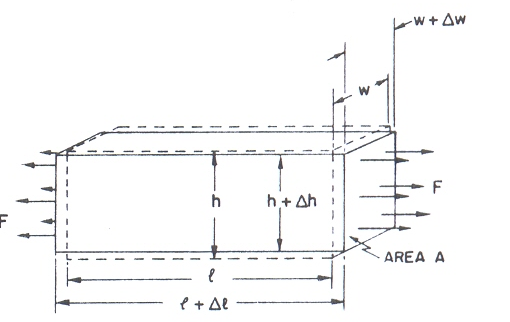
\includegraphics[trim=3mm 3mm 3mm 3mm, clip=true, width=0.8\linewidth]{moduloYoung}
	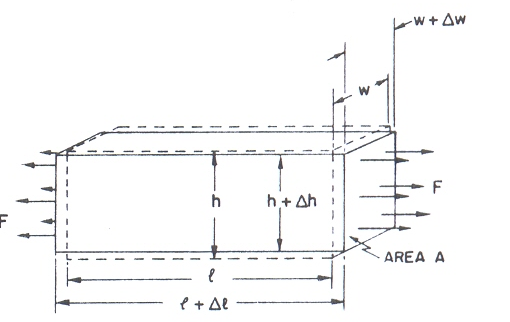
\includegraphics[width=0.8\linewidth]{moduloYoung}
\captionof{figure}{}
\label{fig:fig1}            
%	\caption{Montagem para determinar a Velocidade da Luz. \label{fig:Montagem}} 
\end{center}
%\end{figure}
\end{minipage}
\begin{minipage}[c]{0.4\textwidth}
\begin{equation}
	\label{eq:vc}
	 \frac{F}{A}  = Y  \frac{\Delta l}{l} 
\end{equation}
$Y$ é uma constante de elasticidade, módulo de Young ou de compressão (também representado por $E$) e que tem as dimensões de uma pressão ($Pa$ no SI).
\end{minipage}

Alguns valores típicos para o módulo de Young são dados na tabela
\begin{tabular}{|r|l|}
\hline
\textbf{Material} & \textbf{Y (GPa)}\\
\hline
Borracha & 0.01 - 0.1\\
Nylon & 2 - 4 \\ % \cline{2-2}
Granito & 45 \\
Vidro & 50-90 \\
%\hline \hline
Latão & 50-90 \\
Aço  & 200 \\
Diamante  & 1220 \\
\hline
\end{tabular}

Como consequência da peça alongar e não estar submetida a restrições laterais, nas direções transversais vai observar-se um encurtamento $\Delta h$ e $\Delta w$ que é proporcional a $\Delta l$ mas de sinal contrário, tal que:

\begin{equation}
	\label{eq:poisson}
	 \frac{\Delta w}{w}  =   \frac{\Delta h}{h}  = - \sigma  \frac{\Delta l}{l} 
\end{equation}
em que $\sigma$ (também representado por $\nu$) é outra constante elástica, o \emph{coeficiente de Poisson}, adimensional e que varia no intervalo\footnote{Existe uma clase de materiais, ou estruturas, chamada auxéticos em que o coeficiente de Poisson é negativo.} $[ 0,\;1/2 ] $.
Estas duas constantes elásticas caracterizam todas as propriedades elásticas dos materiais isótropos.

\begin{center}

\begin{tabular}{|r|c|}
\hline
\textbf{Material} & \textbf{$\sigma$}\\
\hline
Cortiça  & $\sim 0.0$ \\
%Nylon & 2 - 4 \\ 
Vidro & 0.18–0.3 \\
Betão & 0.2\\
%Latão & 50-90 \\
Aço  & .3 \\
Borracha & $\sim 0.5$\\
\hline
\end{tabular}
\end{center}


No caso da barra estar submetida a uma pressão idêntica, normal a todas as faces (é o caso de um corpo imerso num fluido submetido à pressão hidrostática) verifica-se uma diminuição de volume que faz intervir uma outra constante de elasticidade, volúmica, $K$ (módulo volúmico de compressão, \emph{“bulk modulus”}). Esta constante pode ser calculada da seguinte forma

\begin{equation}
	\label{eq:bulk}
	 \frac{F}{A}  =  -K \frac{\Delta V}{V} 
\end{equation}
tem as dimensões de uma pressão, não é independente de $Y$ e $\sigma$ e pode provar-se que 

\begin{equation}
	\label{eq:K}
	 K=\frac{Y}{3\,(1-2\sigma)} 
\end{equation}
As forças de compressão ou tração produzem variações de volume sem rotação das partículas do material.

Um meio é considerado anisótropo se as suas propriedades físicas dependem em cada ponto da direção considerada (é o caso dos meios cristalinos). Também os meios amorfos como os vidros, os plásticos, etc. quando são submetidos a esforços adquirem propriedades anisótropas. O carácter anisótropo do material pode ser posto em evidência, por exemplo, colocando-o entre dois polaroides cruzados. Se o material é isótropo a interposição no conjunto dos polaroides não altera a fraca intensidade luminosa, qualquer que seja a sua orientação, em contraste com o que se observa quando o material entre polaroides é anisótropo.

No caso de um meio anisótropo, as elongações para o mesmo esforço mecânico dependem das direções e os diferentes coeficientes de proporcionalidade, i.e., os módulos de elasticidade são elementos do tensor de elasticidade. A caraterização destes materiais exige o conhecimento de um grande número de elementos do tensor ($81=3^4$, que se reduzem a 21 valores independentes).

\subsection{\sf Forças tangenciais }
\begin{center}
	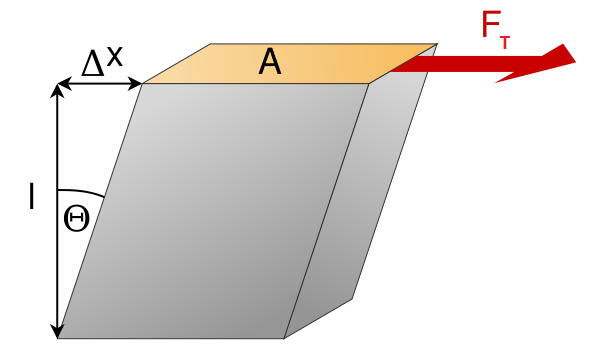
\includegraphics[width=0.45\linewidth]{602px-Shear_scherung}
	\captionof{figure}{\label{fig:fig2}}
\end{center}
Uma barra parelipipédica fixa pela base inferior, se for submetida a um esforço tangencial, como exemplificado na figura \ref{fig:fig2}, deforma-se de modo que as diferentes camadas deslizam umas sobre as outras, não variando o volume. Esse deslize das diferentes camadas pode ser caraterizado pelo ângulo 
$\theta$ que depende da força $F_T$ e da rigidez do material:

\begin{equation}
	\label{eq:shear}
	 \frac{F_T}{A} = \mu \, \theta 
\end{equation}

$\mu$ (também representado por $G$) é o módulo de rigidez (“cisalhamento” ou \emph{“shear modulus”}). Pode provar-se que 
\begin{equation}
	\label{eq:mu}
	 \mu  = \frac{Y}{2(1 +\sigma )}
\end{equation}
Quando as forças tangenciais aplicadas a uma barra cilíndrica, de comprimento $L$ e raio $r$, fixada pela base (situada à esquerda) constituem um binário, por exemplo como o da figura 3, a peça vai torcer.

\begin{center}
	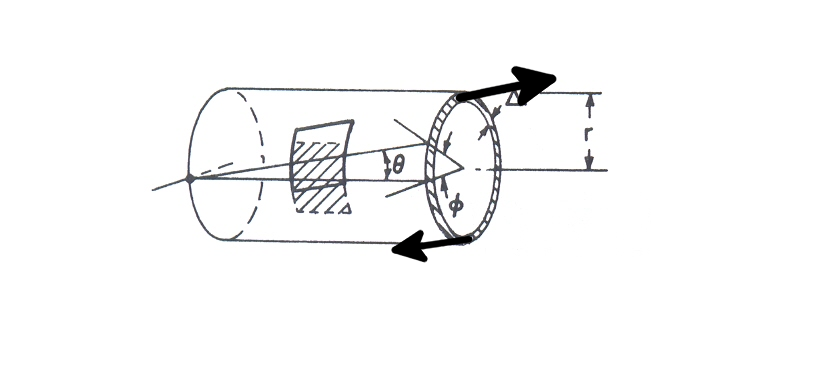
\includegraphics[width=0.5\linewidth]{rotac3}
	\captionof{figure}{\label{fig:fig3}}
\end{center}

Qualquer das geratrizes roda de um ângulo $\theta$ (que satisfaz a equação 	\ref{eq:shear}) e que define na base, onde o binário de forças atua, um ângulo $\Phi$. Esse ângulo depende do momento do binário e da rigidez da peça segundo 
\begin{equation}
	\label{eq:binario}
	 N= \mu \frac{\pi\,r^4}{2\,L} \Phi 
\end{equation}

\subsection{\sf Velocidades de propagação  }

As velocidades das ondas mecânicas que se propagam nos meios sólidos que se comportam como meios elásticos só dependem das constantes de elasticidade e da massa volúmica $\rho$.
Assim, os esforços de compressão/tração produzem ondas longitudinais\footnote{As ondas longitudinais e transversais são referidas, por analogia com as ondas sísmicas, como ondas P (principais) e S (secundárias).} 
%\footnote{As ondas P em sismologia. As Ondas S, são transversais.} 

que se propagam com $v_L$, tendo como suporte o movimento harmónico longitudinal das partículas do meio. Para uma barra 
\begin{equation}
	\label{eq:vL}
	 v_L = \sqrt{\frac{Y}{\rho}}
\end{equation}

No caso de um corpo ie uma peça “volúmica”, em que as distâncias transversais não sejam muito inferiores à distância longitudinal (o comprimento da peça) a expressão (\ref{eq:vL}) tem que ser corrigida de um fator multiplicativo $f$. De facto, o material circundante a cada hipotética barra restringe os movimentos transversais que foram observados na barra (ver equação \ref{eq:poisson}). Nesse caso o módulo de Young vem multiplicado pelo fator

\begin{equation}
	\label{eq:f}
	f = \frac{1-\sigma}{(1+\sigma)(1-2\sigma)} 
\end{equation}
de modo que na equação (\ref{eq:vc}) $Y$ é substituido por $Y'=f\,Y$.

Pode obter-se a expressão que substitui (\ref{eq:vL})  considerando um bloco que é sujeito a compressão/tração mas em que não podem ocorrer contrações laterais. A expressão é a seguinte
\begin{equation}
	\label{eq:vL2}
	 v_L = \sqrt{\frac{K + 4/3\,\mu}{\rho}}
\end{equation}
porque pode mostrar-se facilmente atendendo a (\ref{eq:K}) e (\ref{eq:mu}) que  $Y'=K + 4/3\mu$.

Os esforços tangenciais produzem ondas transversais que se propagam com velocidade $v_T$ graças aos movimentos harmónicos transversais das partículas ou rotações produzidas por um binário de forças. Estas ondas transversais podem vibrar numa determinada direção no plano transversal (fixa ou que segue uma lei de evolução).
% e são pois \emph{polarizáveis}, ao contrário das ondas longitudinais que não são polarizáveis.
\begin{equation}
	\label{eq:vT}
	 v_T = \sqrt{\frac{\mu}{\rho}}
\end{equation}
Para um corpo obtém-se:
\begin{equation}
	\label{eq:v_L_T}
	\left(\frac{v_L}{v_T}\right)^2 =  \frac{2(1-\sigma)}{(1-2\sigma)} 
\end{equation}
que permite a partir da determinação experimental das velocidades $v_L$ e $v_T$ calcular o valor do coeficiente de Poisson $\sigma$. Verifica-se que $v_L$ é sempre superior a $v_T$  (a partir de (\ref{eq:v_L_T}) pode provar-se facilmente que $\sigma<1/2$).
A determinação experimental destas velocidades permite calcular os valores das constantes de elasticidade $K$ e $\mu$, desde que se conheça o valor da massa volúmica do material.

No caso de materiais anisótropos só um grande número de determinações permite calcular as constantes de elasticidade (componentes do tensor de elasticidade). Assim, para um paralelipípedo anisótropo quando se calculam as diferentes velocidades segundo as três direções só é fácil calcular o \emph{coeficiente de anisotropia} $c.a.$ que se obtém pela seguinte expressão
\begin{equation}
	\label{eq:ca}
	c.a.= \frac{v_{max}-v_{min}}{v_{max}}
\end{equation}

\subsubsection{\sf Questões a responder ANTES da sessão de Laboratório}

\begin{enumerate}
\item Para a experiência do Pêndulo e supondo que o fio de Nylon tem um diâmetro de $1\,mm $, calcule a partir da expressão (\ref{eq:vc}), qual a variação de comprimento 
do fio entre a posição mais alta e mais baixa da trajetória. Qual a variação máxima que esta alteração do comprimento provoca no período?
\item Explique a partir das relações (\ref{eq:mu})  e  (\ref{eq:v_L_T})  porque não podem existir ondas transversais em liquídos e gases. Como se pode utilizar esta propriedade 
na exploração de campos de petróleo?
\item Considere uma camada de água, com velocidade de propagação $V_L=1450 \,m/s$, sobre uma camada de rocha granítica (Considere $K_{gra}=50\,GPa$, $\mu_{gra}=24\,GPa$ e \\
$\rho_{gra}=2700\,kg/m^3$). 
Determine o angulo de incidência a partir no qual terá reflexão total das ondas na interface da água para a rocha.
\end{enumerate}

\subsection{\sf Parte experimental }
Nesta experiência vão determinar-se as velocidades de propagação das ondas mecânicas a partir da medida de espaços e tempos em várias amostras cortadas em forma de prisma quadrangular reto, podendo as medidas ser realizadas segundo duas direções ortogonais.
 Calculam-se em seguida as constantes elásticas ($K$, $\mu$ e $\sigma$) para os materiais isótropos e o coeficiente de anisotropia $c.a.$ para os materiais anisótropos.
Dispõe-se de um gerador/recetor que emite impulsos elétricos, que são transformados em impulsos mecânicos por um transdutor piezoelétrico, bem acoplado a uma das faces da amostra. Na face oposta coloca-se outro transdutor, que após a recepção do impulso mecânico o transforma, agora num sinal elétrico e o envia ao gerador/recetor.
O tempo de percurso, que é relativamente curto, porque estas velocidades nos meios sólidos são da ordem do quilómetro por segundo, é determinado com a ajuda dum osciloscópio onde se observam o impulso emitido e o recebido depois de ter sido transmitido através da amostra numa determinada direção. 

\newpage
\section{\sf Protocolo Experimental}
\subsection{\sf Material utilizado}
Conjuntos de sondas Transdutor/Recetor para ondas i) longitudinais e ii)tranversais. Aparelho emissor/recetor de impulsos. Conjunto de cilindros de latão para calibração de sondas. Osciloscópio.
Paquímetro e Balança de pratos

\subsection{\sf Procedimento Experimental}

%As ondas longitudinais e transversais observadas nas amostras são referidas, por analogia com as ondas sísmicas, como ondas P (principais) e S (secundárias).
\begin{enumerate}
\item Começe pelas medidas de calibração dos atrasos no conjunto de amostras de Latão, para as ondas P e S. Represente graficamente os  dados obtidos em função da distância percorrida. Verifique a linearidade e o atraso inicial dos conjunto de medidas (erro sistemático).
\item Para uma amostra isotrópica obtenha as velocidades de propagação(\ref{eq:vL2})  e  (\ref{eq:vT}) nas duas direções perpendiculares à altura dos blocos. 
\item Calculam-se as constantes elásticas ($K$, $\mu$ e $\sigma$) e as respetivas incertezas.
\item Se as velocidades de propagação diferirem de um valor superior aos intervalos de incerteza, calcule o coeficiente de anisotropia.
\end{enumerate} 


\section*{\sf Apêndice}
\subsection{\sf A equação de propagação por ondas (ondas planas)} 

Foi apresentada nas Aula Teóricas a forma de um campo vetorial $\vec{V}$ organizado em onda plana 
\begin{equation}
	\label{eq:onda}
	\vec{V}(x,t)=\vec{V}_{max} \sin \left(\frac{2\,\pi}{T} - \frac{2\,\pi}{\lambda} + \delta \right)
\end{equation}

A fase da onda $\phi = \frac{2\,\pi}{T}\,t - \frac{2\,pi}{\lambda}\,x + \delta$  é o argumento da função trigonométrica e contém os parâmetros que caraterizam a periodicidade da onda $T$ e $λ$ e ainda a desfasagem $δ$ que dá conta do valor da amplitude no início do tempo e do espaço. Para simplificar, vamos considerar $δ=0$ e só a intensidade do campo.

A velocidade de fase $v_{ph}$ é definida como a velocidade tal que a fase seja constante, ie,  $v_{ph}=(\frac{\ud x}{\ud t})_{\ud \phi=0}$

A partir de $\ud \phi = 0 \Rightarrow \frac{2\,\pi}{T}\,\ud t - \frac{2\,\pi}{\lambda}\,\ud x$  obtém-se

\begin{equation}
	\label{eq:v}
	v=\frac{\lambda}{T} 
\end{equation}

Calculando $\frac{\partial V }{\partial x}, \;\frac{\partial V }{\partial x}, \;\frac{\partial^2 V }{\partial x^2}, \; \textrm{ e } \;\frac{\partial^2 V }{\partial t^2} $   e    obtém-se\footnote{Para simplificação da escrita usa-se $V$ em vez de $\vec{V}$. }

\begin{IEEEeqnarray}{lCr}
\frac{\partial V }{\partial x} = V_{max} \, (-\frac{2\,\pi}{\lambda}) \cos \phi &\qquad& \frac{\partial V }{\partial t} = V_{max} \, (+\frac{2\,\pi}{T}) \cos \phi\\
%
\frac{\partial^2 V }{\partial x^2} = -V_{max} \, \left(-\frac{2\,\pi}{\lambda}\right)^2 \sin \phi &\qquad& \frac{\partial^2 V }{\partial t^2} = -V_{max} \, \left(+\frac{2\,\pi}{T}\right)^2 \sin \phi
\end{IEEEeqnarray}

A partir das duas últimas expressões 

\begin{equation}
	\label{eq:ondap}
-V_{max} (2 \pi)^2  \sin \phi = \lambda^2 \frac{\partial^2 V }{\partial x^2} = T^2 \, \frac{\partial^2 V }{\partial t^2} \Rightarrow 
\frac{\partial^2 V }{\partial x^2} = \frac{1}{v^2}  \, \frac{\partial^2 V }{\partial t^2}
\end{equation}

Esta última equação é a equação diferencial caraterística das ondas planas que põe em evidência a velocidade de propagação de fase $v$. Qualquer campo escalar ou vetorial organizado em onda plana satisfaz a uma equação deste tipo.

\subsection{\sf A equação de propagação das ondas longitudinais nos sólidos} 

Consideremos agora uma fatia elementar de uma barra cilíndrica de um material de massa volúmica $\rho$, de seção $A$e espessura $\ud x$, submetida a duas forças de compressão normais à seção, numa face $F$ e na outra $F+\ud F$. Esta diferença $\ud F$ produz um deslocamento  $\ud \xi$  segundo o eixo do cilíndro.

A equação (\ref{eq:vc}) escreve-se agora em termos do deslocamento elementar da seguinte forma
\begin{equation}
	\label{eq:a4}
	 F = A \, Y \frac{\partial \xi }{\partial x} 
\end{equation}

A força $ \ud F = \frac{\partial F }{\partial x} \ud x $   produz uma aceleração $\frac{\partial^2 \xi }{\partial t^2} $  sobre a massa elementar da fatia $\ud m= \rho\,A \ud x $  tal que pela lei de Newton

\begin{equation}
	\label{eq:a5}
	 \frac{\partial F }{\partial x} \ud x  =  \rho\,A \ud x \frac{\partial^2 \xi }{\partial t^2} \Rightarrow \frac{\partial F }{\partial x} = \rho\,A  \frac{\partial^2 \xi }{\partial t^2}
\end{equation}

Aplicando a derivada parcial em ordem a $x$ à equação (\ref{eq:a4}) obtém-se
\begin{equation}
	\label{eq:a6}
	\frac{\partial F }{\partial x} = A \, Y \frac{\partial^2 \xi }{\partial x^2}
\end{equation}	

Combinando (\ref{eq:a5}) e (\ref{eq:a6}) obtemos a equação :
\begin{equation}
	\label{eq:a7}
	\frac{\partial^2 \xi }{\partial x^2} - \frac{\rho}{Y} \frac{\partial^2 \xi }{\partial t^2} =0
\end{equation}	

Esta equação é caraterística duma onda plana que se propaga com velocidade $v_{ph}=\sqrt{\frac{Y}{\rho}}$  , velocidade que corresponde à velocidade longitudinal apresentada na equação (\ref{eq:vL}). 

\end{document} 